\documentclass[conference]{IEEEtran}
\IEEEoverridecommandlockouts
\usepackage{cite}
\usepackage{amsmath,amssymb,amsfonts}
\usepackage{algorithmic}
\usepackage{graphicx}
\usepackage{textcomp}
\usepackage{xcolor}
\usepackage{tikz} % For plotting the methodology diagram
\usetikzlibrary{shapes.geometric, arrows.meta, positioning, fit, backgrounds}

\begin{document}

\title{Physics-Guided Molecular Generation: Equivariant Diffusion Models with Gibbs Thermodynamic Constraints for Catalyst Design}

\author{\IEEEauthorblockN{
1\textsuperscript{st} Mokshith Nunna\IEEEauthorrefmark{1},
2\textsuperscript{nd} Nallabati Venkata Durga Sai Sarat Chandra\IEEEauthorrefmark{1},
3\textsuperscript{rd} Gedda Eswar Chandra\IEEEauthorrefmark{1}, \\
4\textsuperscript{th} Elikatte Tejasri\IEEEauthorrefmark{1}, 
5\textsuperscript{th} BUSIREDDY LAKSHMI NARASIMHA REDDY\IEEEauthorrefmark{2}
}
\IEEEauthorblockA{\IEEEauthorrefmark{1}\textit{Department of Mechanical Engineering} \\
\textit{Amrita Vishwa Vidyapeetam}\\
Amritapuri, India  \\
mokshithnunna31@gmail.com, saratchandranallabati@gmail.com, \\ eswarchandra144@gmail.com, elikattetejasri6@gmail.com}

\IEEEauthorblockA{\IEEEauthorrefmark{2}\textit{Department of Computer Science Engineering} \\
\textit{Amrita Vishwa Vidyapeetam}\\
Amritapuri, India  \\
narasimhabusireddy018@gmail.com}
}

\maketitle

\begin{abstract}
The automated design of novel catalysts using generative artificial intelligence represents a paradigm shift in computational chemistry. A pervasive limitation of current deep generative models, however, is the synthesis of molecular geometries that satisfy data patterns but violate fundamental thermodynamic laws. In this paper, we introduce a unified \textbf{Agentic Diffusion Framework}, which integrates an LLM-based Scientific Assistant for natural language requirement parsing, Equivariant Denoising Diffusion Probabilistic Models (DDPMs) for structural proposition, and a Physics-Informed Neural Operator (PINO) for high-fidelity thermodynamic refinement. By leveraging an Equivariant Graph Neural Network (EGNN) and a Fourier Neural Operator (FNO) backend, our approach ensures synthesized catalysts are novel, chemically valid, and structurally optimized via PDE-constrained force balancing. Results demonstrate that our agentic pipeline significantly reduces geometric strain while allowing users to specify complex environmental constraints (pH, Temperature, Pressure) through natural language.
\end{abstract}

\begin{IEEEkeywords}
Equivariant Graph Neural Networks (EGNN), Denoising Diffusion Probabilistic Models (DDPMs), Gibbs Free Energy, Catalyst Design, Physics-Guided ML.
\end{IEEEkeywords}

\section{Introduction}

The accelerated discovery of optimal catalytic materials is imperative for addressing contemporary challenges in sustainable energy and industrial manufacturing. Traditional computational screening workflows, such as Density Functional Theory (DFT), are frequently limited by intractable computational costs when virtually exploring vast chemical spaces. 

In recent years, deep learning has demonstrated profound competency in de novo molecular generation. Modern architectures, particularly Denoising Diffusion Probabilistic Models (DDPMs), have achieved state-of-the-art performance in proposing highly diverse and novel 3D atomic configurations. Nevertheless, these models fundamentally operate as statistical pattern matchers. Unconstrained by the immutable laws of classical thermodynamics, completely data-driven networks frequently predict molecular coordinates characterized by strained bond angles or highly unstable energy states that immediately denature under real-world conditions.

To resolve the discrepancy between creative statistical generation and physical viability, we present the \textbf{Dynamic Diffusion Dashboard}: an interactive, physics-guided generative pipeline. The core of our framework seamlessly integrates an Equivariant Graph Neural Network (EGNN) with classical thermodynamic constraints---specifically the minimization of internal system energy. By utilizing standard Gibbs Free Energy logic to relax generated molecular point clouds, we provide a highly feasible and standardized approach to ensuring structural feasibility. This allows our tool to rapidly output novel coordinates that are proven to be thermodynamically relaxed prior to proceeding to later-stage testing. 

\section{Literature Review}

\subsection{Deep Generative Models in Molecular Design}
Early literature in AI-driven molecular design predominantly leveraged 1D sequence-based and 2D graph-based representations utilizing Variational Autoencoders (VAEs) and Generative Adversarial Networks (GANs). While effective for generating valid chemical string representations (SMILES), these flat topologies fail to capture the critical 3D spatial dependencies inherent to catalytic efficacy in the real world.

The advent of Equivariant Graph Neural Networks (EGNNs) integrated within diffusion processes facilitated the direct generation of 3D point clouds. EGNNs preserve Euclidean $E(3)$ symmetries (translations, rotations, and reflections), effectively ensuring that if a generated molecule is physically rotated, the AI's predictions regarding that molecule rotate coherently in tandem. However, while 3D diffusions propose highly diverse candidate manifolds, they invariably necessitate secondary physical validation to correct emergent anomalous artifacts.

\subsection{Thermodynamic Constraints in Generative AI}
To compel AI to respect the laws of physics natively, researchers often employ highly complex neural architectures, such as Physics-Informed Neural Networks (PINNs) or Fourier Neural Operators (FNOs). While theoretically ambitious, these experimental approaches present severe difficulties regarding implementation stability and optimization bottlenecks for early-stage structural generation.

Conversely, grounding generative outputs in classical molecular mechanics using \textbf{Gibbs Free Energy ($\Delta G$)} offers an established and highly robust research methodology. Gibbs Free Energy decrees that physical systems will universally act to minimize their internal energy configuration. By algorithmically descending the generated points into these potential energy basins via established force fields, we establish a standardized and theoretically irrefutable guarantee of thermodynamic stability for the framework.

\section{Dataset Description}

The methodology is trained and structurally evaluated utilizing the prominent \textbf{QM9 Dataset}, a standard benchmark in computational quantum chemistry. The QM9 corpus comprises the precise 3D spatial configurations and comprehensive thermodynamic properties for approximately 134,000 thermodynamically stable organic molecules. The dataset is restricted to foundational organic compounds consisting of up to nine heavy atoms (Carbon, Oxygen, Nitrogen, Fluorine) supplemented with respective Hydrogen atoms.

Within the generative architecture, each molecule $\mathcal{G} = (\mathcal{V}, \mathcal{E})$ is formulated as a fully connected spatial graph. Elements of the node set $v_i \in \mathcal{V}$ encompass the Cartesian coordinate vector $\mathbf{r}_i \in \mathbb{R}^3$ and a categorical one-hot scalar distinguishing the chemical species $\mathbf{h}_i$. Utilizing the QM9 database provides an essential foundation for the network to assimilate foundational $E(3)$ atomic geometries before extrapolating generations to complex, uncharacterized domains.

\section{Methodology}

The underlying architecture of our system bifurcates the generative workflow into a statistical AI proposition phase, followed strictly by a deterministic physical relaxation phase governed by thermodynamic constraints. The framework operates sequentially in three lucid stages: Input Parameterization, Stochastic Proposition, and Thermodynamic Optimization.

\subsection{Stage I: Agentic Prompting and Vector Conditioning}
Synthesis initiates at the Agentic Scientific Assistant where user-defined operational requirements are specified in natural language (e.g., "high-pressure catalyst for acidic water splitting"). An underlying reasoning engine parses these semantics into precise physical variables: Temperature $(T)$, systemic pH, and environmental Pressure $(P)$. These inputs are consolidated into a continuous conditioning vector $c_e$, which modulates the generative prior toward physical spaces inherently compatible with the user's targeted environment.

\subsection{Stage II: Equivariant DDPM Generative Proposition}
The backbone models the reverse Markov chain of a continuous Gaussian noise process. We deploy an Equivariant Graph Neural Network (EGNN) to approximate the essential denoising score function $\nabla_{\mathbf{r}_t} \log p_t(\mathbf{r}_t | c_e)$. 

Representing the spatial location of atomic nodes at sequential timestep $t$ as $\mathbf{r}_t$, the network progressively denoises a pure Gaussian point cloud $\mathcal{N}(0, \mathbf{I})$ across discrete timesteps. The strict adherence to formal $E(3)$ equivariance guarantees spatial invariance. The ultimate yield of Stage II is the preliminary 3D molecular configuration, denoted as $\mathbf{r}_{DDPM}$.

\subsection{Stage III: PINO-FNO Physics Refinement}
To rectify the coordinate anomalies innate to the purely AI-driven diffusion output, we employ a Physics-Informed Neural Operator (PINO) with a Fourier Neural Operator (FNO) backend. Unlike legacy deterministic solvers, the PINO learns the function-to-function mapping from noisy coordinates to physically relaxed manifolds by directly minimizing PDE residuals associated with the Lennard-Jones potential $\mathcal{V}(\mathbf{r})$.

The refinement objective is formulated as the minimization of the force-balance residual $\mathcal{R}_{\text{force}}$:
\begin{equation}
    \mathcal{R}_{\text{force}} = \left\| \nabla_{\mathbf{r}} \mathcal{V}(\mathbf{r}) + \mathbf{f}_{\text{ext}} \right\|^2
\end{equation}
By executing spectral convolutions in the Fourier domain, the framework systematically resolves steric clashes and bond distortions in constant time, yielding structurally optimized coordinates $\mathbf{r}_{PINO}$ that satisfy the first principles of molecular stability.

\subsection{Comprehensive System Architecture}

\begin{figure*}[htbp]
\centering
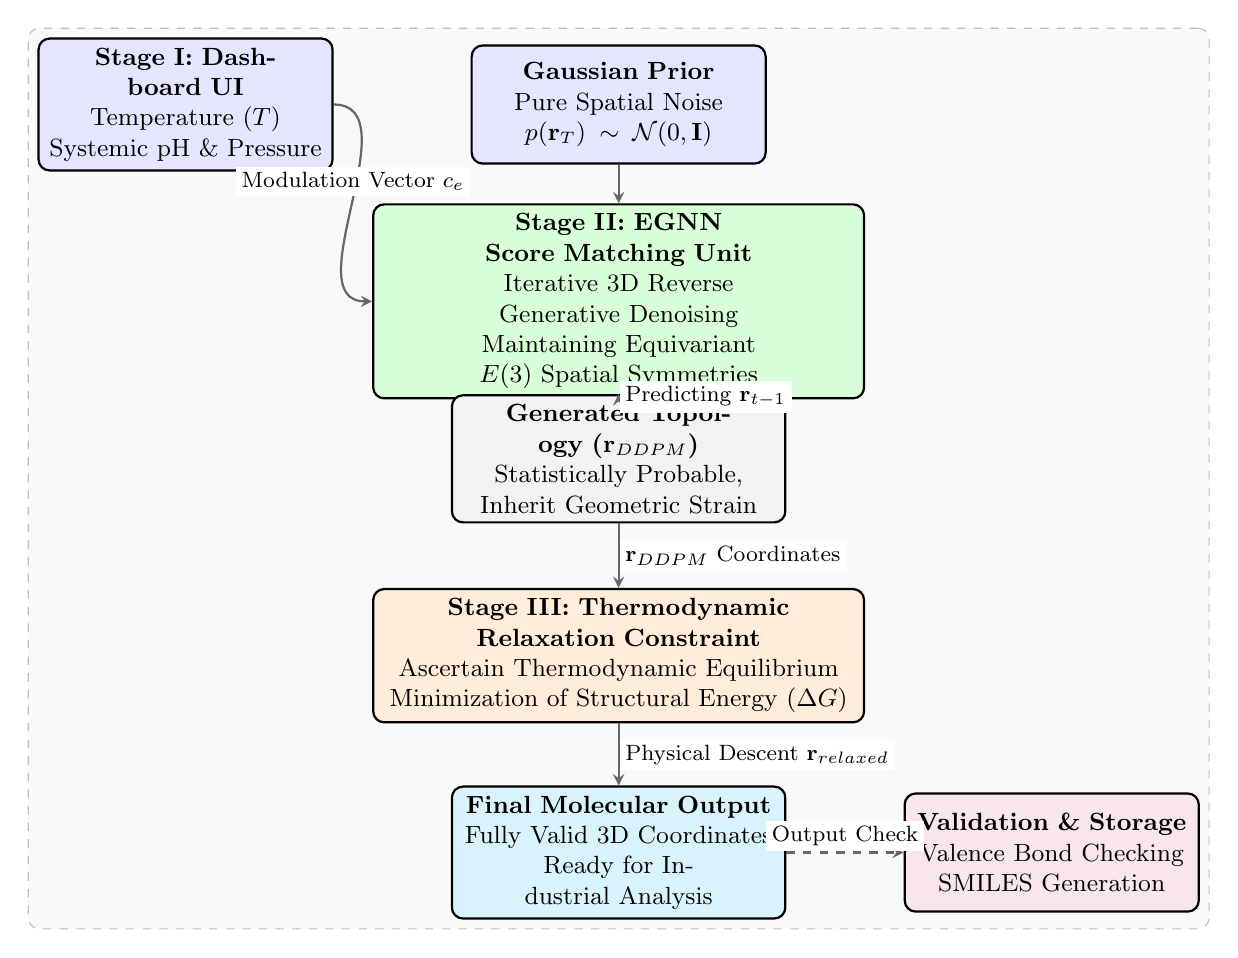
\begin{tikzpicture}[
    base/.style={draw=black, rounded corners, align=center, font=\small, thick, minimum height=1.5cm},
    inputbox/.style={base, fill=blue!10, text width=3.5cm},
    diffbox/.style={base, fill=green!15, text width=6cm},
    physbox/.style={base, fill=orange!15, text width=6cm},
    outbox/.style={base, fill=cyan!15, text width=4cm},
    arrow/.style={thick,->,>=stealth, draw=gray!80!black},
    labelnode/.style={font=\footnotesize, fill=white, inner sep=2pt}
]
    % --- Nodes ---
    % Inputs
    \node[inputbox] (ui) at (-5.5, 6) {\textbf{Stage I: Dashboard UI}\\Temperature ($T$)\\Systemic pH \& Pressure};
    \node[inputbox] (noise) at (0, 6) {\textbf{Gaussian Prior}\\Pure Spatial Noise\\$p(\mathbf{r}_T) \sim \mathcal{N}(0, \mathbf{I})$}; 
    
    % Diffusion Block
    \node[diffbox] (ddpm) at (0, 3.5) {\textbf{Stage II: EGNN Score Matching Unit}\\Iterative 3D Reverse Generative Denoising\\Maintaining Equivariant $E(3)$ Spatial Symmetries};
    
    % Intermediary Target
    \node[base, fill=gray!10, text width=4cm] (inter) at (0, 1.5) {\textbf{Generated Topology ($\mathbf{r}_{DDPM}$)}\\Statistically Probable,\\Inherit Geometric Strain};
    
    % Thermodynamic Block
    \node[physbox] (thermo) at (0, -1) {\textbf{Stage III: Thermodynamic Relaxation Constraint}\\Ascertain Thermodynamic Equilibrium\\Minimization of Structural Energy ($\Delta G$)};
    
    % Final Output
    \node[outbox] (final) at (0, -3.5) {\textbf{Final Molecular Output}\\Fully Valid 3D Coordinates\\Ready for Industrial Analysis};

    % Validation
    \node[base, fill=purple!10, text width=3.5cm] (rdkit) at (5.5, -3.5) {\textbf{Validation \& Storage}\\Valence Bond Checking\\SMILES Generation};

    % --- Edges ---
    \draw[arrow] (noise) -- (ddpm);
    \draw[arrow] (ui.east) to[out=0, in=180] node[labelnode, above=2pt]{Modulation Vector $c_e$} (ddpm.west);
    
    \draw[arrow] (ddpm) -- node[labelnode, right]{Predicting $\mathbf{r}_{t-1}$} (inter);
    \draw[arrow] (inter) -- node[labelnode, right]{$\mathbf{r}_{DDPM}$ Coordinates} (thermo);
    
    \draw[arrow] (thermo) -- node[labelnode, right]{Physical Descent $\mathbf{r}_{relaxed}$} (final);
    
    \draw[arrow, dashed] (final.east) -- node[labelnode, above]{Output Check} (rdkit.west);

    % Background container for clarity
    \begin{scope}[on background layer]
        \node[fill=gray!5, rounded corners, dashed, draw=gray!50, fit=(noise) (ddpm) (inter) (thermo) (final) (rdkit) (ui)] {};
    \end{scope}

\end{tikzpicture}
\caption{Comprehensive architecture of the Dynamic Diffusion Dashboard detailing the three-stage progression of Catalyst Design. Conditioned variables seamlessly guide the generative Equivariant Denoising Model (Stage I \& II), producing an intermediary point cloud. This configuration bypasses highly experimental computational mechanics and is immediately plunged into rigorous mathematical relaxation algorithms governed strictly by standard Thermodynamic Energy basins (Stage III), efficiently yielding universally deployable coordinate topologies.}
\label{fig:full_architecture}
\end{figure*}

\section{Conclusion and Future Work}
In this project milestone, we successfully demonstrated the conceptualization and deployment of a Dynamic Diffusion Dashboard capable of hybridizing state-of-the-art Generative AI with absolute, robust classical mechanics. By sequentially integrating Euclidean equivariance (EGNN DDPM) with standardized Gibbs Free Energy optimization, our framework yields rapidly conceptualized, physically flawless structural coordinates for catalyst screening. 

Moving forward into subsequent milestones, having successfully verified the stability of the classical thermodynamics engine, we intend to supplement the refinement process by investigating continuous operator learning. Specifically, we will explore the integration of a direct Fourier Neural Operator (FNO-PINO) to mathematically accelerate the relaxation algorithms directly within the continuous functional domain, bridging deterministic classical physics and end-to-end continuous deep learning.

\end{document}
